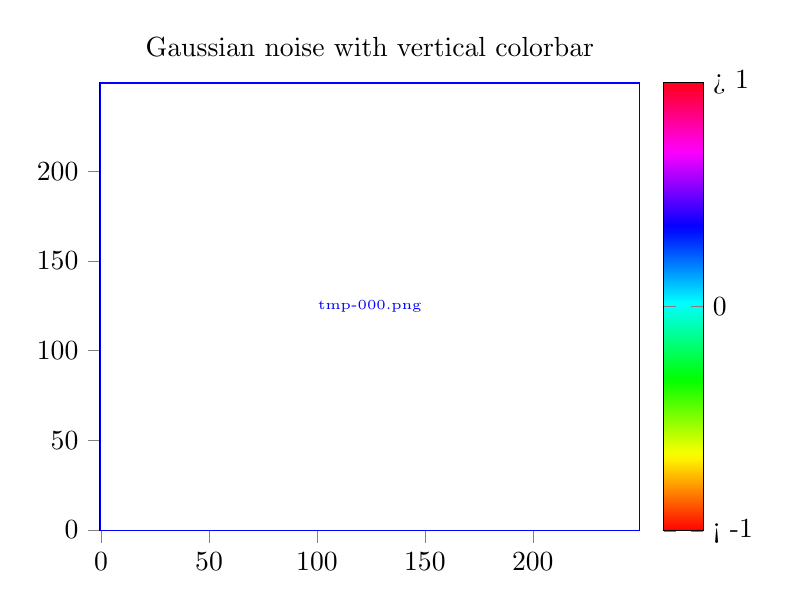
\begin{tikzpicture}

\begin{axis}[
colorbar,
colorbar style={ytick={-1,0,1},yticklabels={< -1,0,> 1},ylabel={}},
colormap={mymap}{[1pt]
  rgb(0pt)=(1,0,0);
  rgb(10pt)=(1,0.9375,0);
  rgb(11pt)=(0.96875,1,0);
  rgb(21pt)=(0.03125,1,0);
  rgb(22pt)=(0,1,0.0625);
  rgb(32pt)=(0,1,1);
  rgb(42pt)=(0,0.0625,1);
  rgb(43pt)=(0.03125,0,1);
  rgb(53pt)=(0.96875,0,1);
  rgb(54pt)=(1,0,0.9375);
  rgb(63pt)=(1,0,0.09375)
},
point meta max=1,
point meta min=-1,
tick align=outside,
tick pos=left,
title={Gaussian noise with vertical colorbar},
x grid style={white!69.01960784313725!black},
xmin=-0.5, xmax=249.5,
y grid style={white!69.01960784313725!black},
ymin=-0.5, ymax=249.5
]
\addplot graphics [includegraphics cmd=\pgfimage,xmin=-0.5, xmax=249.5, ymin=249.5, ymax=-0.5] {tmp-000.png};
\end{axis}

\end{tikzpicture}